\section{Route 1: Fahrradtunnel Universitäten}
Folgende Route schlagen wir als Hauptverbindung im Grazer Osten in Tunnelform vor:

\begin{itemize}
    \item Inffeldgasse
    \item Neue Technik
    \item Alte Technik
    \item Lichtenfelsgasse
    \item KFU Hauptgebäude (Kreuzung mit Route 2)
    \item Kreuzschwestern-Park
    \item Wirtschaftskammer/Campus02
\end{itemize}

\begin{figure}
    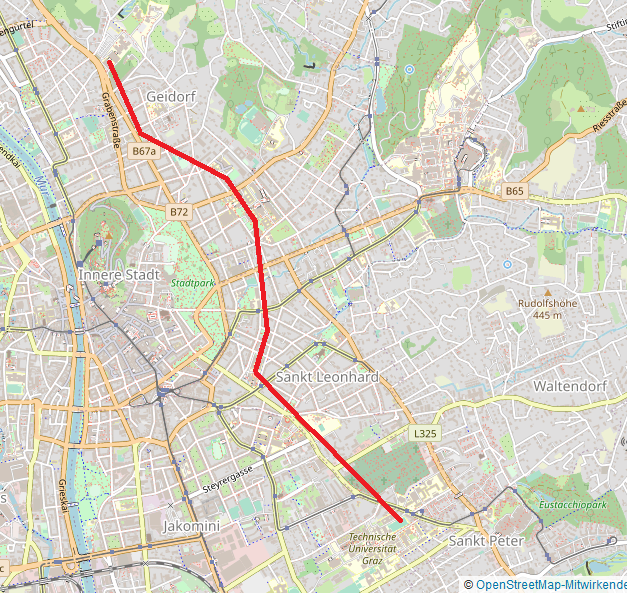
\includegraphics[width=0.8\textwidth]{main/bike/tunnel/uni/linie1}
    \centering
    \caption[Verlauf Linie 1]{Verlauf der Linie 1 zwischen den Zufahrten}
\end{figure}

Zwischen den einzelnen Universitäten findet oft besonders reger Radverkehr statt, und auf dieser Achse ist aufgrund der Bauweise der Stadt oft besonders wenig Platz für Radinfrastruktur.

Dieser Tunnel stellt eine Achse Nord-Süd dar und ist mit einer Kreuzung sowohl mit dem Stadtzentrum als auch dem Landeskrankenhaus verbunden.

\subsection{Zufahrt Inffeldgasse}

\subsection{Mögliche Verlängerung nach Süden}
Von der Zufahrt Inffeldgasse aus ist eine Verlängerung nach Süden denkbar mit folgenden weiteren Zufahrten:
\begin{itemize}
    \item ORF-Park
    \item Wohnpark St. Peter
    \item Messendorf
    \item Raaba
\end{itemize}

\subsection{Mögliche Verlängerung nach Norden}
Von der Zufahrt Wirschaftskammer aus ist eine weitere Verlängerung in Richtung Norden denkbar mit folgenden weiteren Zufahrten:
\begin{itemize}
    \item Ortweinschule
\end{itemize}

Von dort aus ist das Radwegenetz auch oberirdisch gut möglich und teilweise bereits ausgebaut.